\section{Introduction - p-B$^{11}$ Fusion}
\begin{frame} {p-B$^{11}$ as Fusion Fuel}
    Advantages:
    \begin{itemize}
        \item No neutrons are produced in this reaction, p+B$^{11}\to$ 3He$^4$.
        \item Released energy is carried only by charged particles.
        \item No need to use heat-exchanger, charged particles create electricity directly.
        \item Only tiny amount of neutrons is produced in secondary reaction, He$^4$+B$^{11}\to$N$^{14}$+n.
        \item No radioactive waste.
    \end{itemize}

    Challenges:
    \begin{itemize}
        \item Requires average ion energies above 100\unit{\kilo\eV}. (DT fusion requires 40\unit{\kilo\eV}).
        \item Plasma density-confinement product $n\tau$ requirement is 15 times higher than DT fusion.
        \item Boron ions lead far greater amounts of X-ray energy than DT fusion.
    \end{itemize}
\end{frame}

\begin{frame} {Dense Plasma Focus (DPF)}
    Advantages:
    \begin{itemize}
        \item Extremely compact.
        \item Simple in construction.
        \item No need for external magnets nor lasers.
        \item Utilize the instabilities of plasma rather than fighting them.
    \end{itemize}

    Challenges:
    \begin{itemize}
        \item Very bad fusion yield, efficiency $1.25\times10^{-5}$.
    \end{itemize}
\end{frame}

\begin{frame} {Fusion Yield}
    \begin{figure}
        \centering
        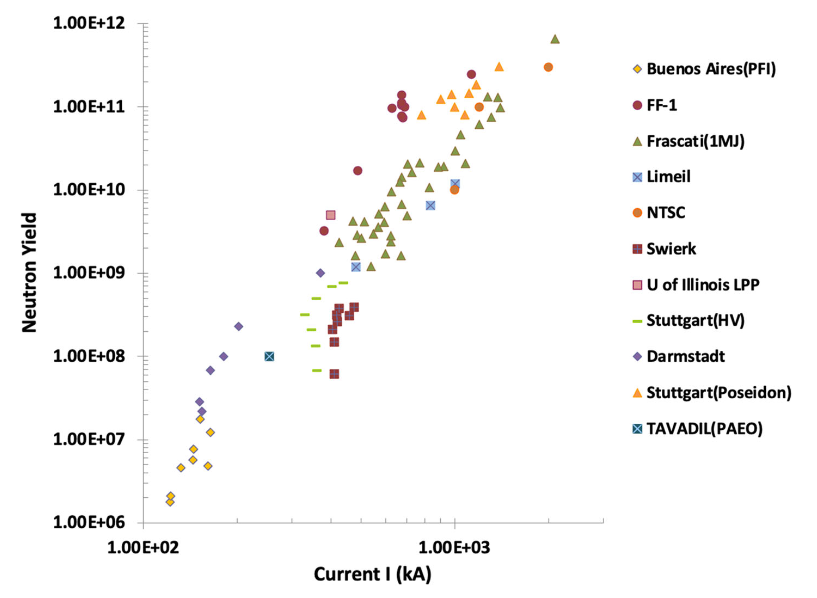
\includegraphics[width=0.45\textwidth]{figures/fusion-yield.png}
        \caption{Up to peak currents of 1MA, DPF fusion yield rises sharply with increasing current, but plateaus above 1MA. At lower currents, FF-1's performance exceeds those of other DPFs, but was comparable to other best results at 1MA. \cite{lerner_2023_focus}}
        \label{fig:fusion-yield}
    \end{figure}

    E. J. Lerner, S. M. Hassan, I. Karamitsos-Zivkovic, and R. Fritsch. Focus Fusion: Overview of Progress Towards p-B11 Fusion with the Dense Plasma Focus.
\end{frame}